In an attempt to homogenise the figures obtained with ParaView, I have decided to use 
a fixed colour scale for each field throughout this document. These colour scales were 
obtained from \url{https://peterkovesi.com/projects/colourmaps} and are 
Perceptually Uniform Colour Maps \cite{kove15}. 

\begin{center}
\begin{tabular}{lll}
\hline
Field & colour code & \\
\hline\hline
Velocity/displacement & CET-D1A & 
\includegraphics[width=3cm]{images/colourscales/CET-D1A}\\
\hline
Pressure& CET-L17 & 
\includegraphics[width=3cm]{images/colourscales/CET-L17}\\
\hline
Velocity divergence& CET-L1 & 
\includegraphics[width=3cm]{images/colourscales/CET-L1}\\
\hline
Density& CET-D3 & 
\includegraphics[width=3cm]{images/colourscales/CET-D3}\\
\hline
Strain rate& CET-R2 & 
\includegraphics[width=3cm]{images/colourscales/CET-R2}\\
\hline
Viscosity & CET-R3 & 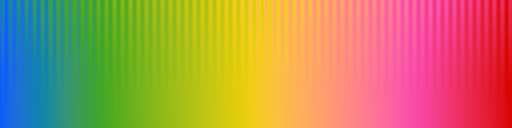
\includegraphics[width=3cm]{images/colourscales/CET-R3}\\
\hline
Temperature & CET-D9 & 
\includegraphics[width=3cm]{images/colourscales/CET-D9}\\
\hline
stress & CET-L18 &  
\includegraphics[width=3cm]{images/colourscales/CET-L18}\\
\hline
Spin tensor & CET-R1 &  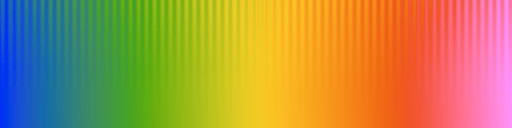
\includegraphics[width=3cm]{images/colourscales/CET-R1}\\
\hline
Composition field & CET-CBD1 &  
\includegraphics[width=3cm]{images/colourscales/CET-CBD1}\\
\hline
\end{tabular}
\end{center}

%https://peterkovesi.com/projects/colourmaps/




